\documentclass{article}
\usepackage{tikz}
\usetikzlibrary{matrix}

\begin{document}

\begin{figure}[h]
    \centering
    \begin{tikzpicture}[scale=0.8]
        % Define the nodes for the small boxes (daily routing and scheduling problems)
        \foreach \x in {1,...,3} {
            \foreach \y in {1,...,3} {
                \node[draw] (small-\x-\y) at (\x,\y) {};
            }
        }
        
        % Define the nodes for the large boxes (multi-day solutions)
        \foreach \x in {1,...,2} {
            \foreach \y in {1,...,2} {
                \node[draw] (large-\x-\y) at (\x*4+1,\y*3+1) {};
            }
        }
        
        % Draw the lines connecting the small boxes to the large boxes
        \draw (small-1-1) -- (large-1-1);
        \draw (small-1-2) -- (large-1-1);
        \draw (small-1-3) -- (large-1-1);
        \draw (small-2-1) -- (large-1-2);
        \draw (small-2-2) -- (large-1-2);
        \draw (small-2-3) -- (large-1-2);
        \draw (small-3-1) -- (large-2-1);
        \draw (small-3-2) -- (large-2-1);
        \draw (small-3-3) -- (large-2-1);
        
        % Add the text description
        \node[anchor=south west, inner sep=0pt] at (current bounding box.north west) {
            \textmd{Two-fold decomposition of the problem structure. The small boxes represent daily routing and scheduling problems for each caregiver. The daily solutions for each caregiver are combined to create multi-day solutions, represented by the large boxes. The corresponding combination process ensures that the required number of treatments is met, and the minimum number of days between two visits is satisfied. The multi-day plans for each caregiver are further combined to ensure strict continuity of care and minimize overall cost.}
        };
    \end{tikzpicture}
\end{figure}

\end{document}